%% The end to end process: second chapter.

\chapter{End to End: From Source to e-reader}

We'll start with the end-to-end process for making a book you can read
on your e-reader device. Checking that you can do this, change the title,
add or remove chapters, and see the changes you've made reflected on your 
e-reader, will hopefully be the best encouragement to work through more
of this book, focusing on the topics that are most useful for your own book.

\begin{figure}
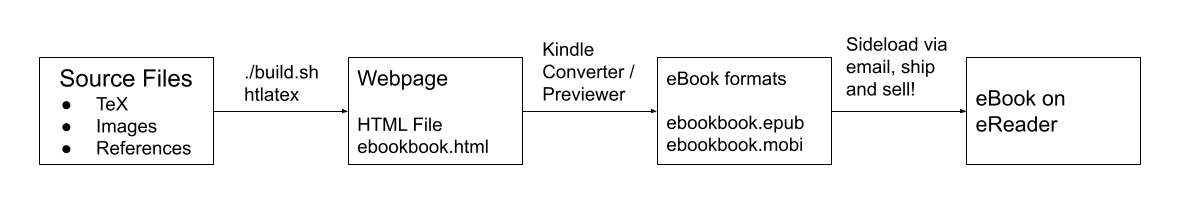
\includegraphics[width=\linewidth]{images/pipeline.png}
\caption{Steps in the pipeline for shipping this ebook}
\label{fig:pipeline}
\end{figure}

The basic outline of the process is shown in Figure \ref{fig:pipeline}.
The rest of this chapter serves to describe the steps in more detail.

The descriptions of commands here will be relatively high-level ---
we'll say things ``install git and run git clone'', rather than giving
details on how to do this on various operating systems. This is for
three reasons. The first is that it's easier to write instructions
this way. The second is that very specific instructions of which web
addresses to visit and which buttons to click on can go stale very
quickly. The third is that this book does assume that the reader has
some experience with and / or tolerance for figuring out a certain
amount of installation and troubleshooting on computers. If not, there are
more constrained off-the-shelf tool that will be easier to get started with
than \latex.

%%
\section{Access and Build the \latex Source}

First of all, you'll want to get a copy of the source code for this
book. (We won't split hairs about whether \latex sources count as
`code'. It gives instructions to machines, it's easy to make mistakes
that show up as error messages, and it's reviewed and stored in source
control --- so it's like code in these practical senses.)

If you already have \texttt{git} installed, this will be something
like running \texttt{git clone
  https://github.com/dwiddows/ebookbook.git} at a command prompt, or
downloading the code using some visual client software. 

List the contents of this directory and check that you can see the
files \texttt{ebookbook.tex} and \texttt{build.sh}. The first of these
is the main \tex document that lays out how to combine the other files
into an ebook.  The second is a build script --- on platforms with
bash or a compatible shell installed, you should be able to run just
\texttt{./build.sh} and get most of the book built using one
command. Or at least, to begin with, you should get error messages
telling you if anything is missing and needs to be installed. If you're not
running a compatible shell, the \texttt{build.sh} will at least give a list
of commands you'll need to run some other way.

So the next step is to run \texttt{./build.sh} and ideally it should
typeset a copy of this book.

%%
\section{From HTML to ePub ... or Mobi}

The most important output from the previous step is a file called \texttt{ebookbook.html}.
This is really formatted for display as a webpage in a browser. This is different
from the more common use of \tex to make documents such as academic papers, which are
nowadays normally created as PDF files.


